\documentclass{beamer}

%\usetheme{ENSLyon}

\usetheme{AnnArbor}

\title[SIC 2018]{\Large Complexidade Computacional do PGDM}
\author[G. Philippi]{{\bf Guilherme Philippi}}
\institute[]{Acadêmico de Engenharia de Controle e Automação\\ Campus Blumenau \\  Universidade Federal de Santa Catarina \\ UFSC\\ Orientado por Felipe Delfini Caetano Fidalgo \vspace{0.3cm}}
\date[04 de Outubro, 2018]{\scriptsize SIC 2018 \\ Seminário de Iniciação Científica \\ Blumenau - Santa Catarina - Brasil}
\setbeamersize{text margin left=5mm}
\setbeamersize{text margin right=5mm}

\setbeamertemplate{navigation symbols}{}
%\usecolortheme{ENSLyon_greener}
\usecolortheme{wolverine}

%PACKAGES -------------------------
\usepackage{etex}
\usepackage[utf8]{inputenc}
\usepackage[english]{babel}
\usepackage{enumerate}
\usepackage{amsmath}
\usepackage{amssymb}
\usepackage{amsthm}
\usepackage{amscd}
\usepackage{amsfonts}
\usepackage{multicol}
\usepackage{multirow}
\usepackage{array}
\usepackage{color}
\usepackage{graphicx}
\usepackage{tikz}
\usepackage{tikz-qtree}
\usepackage{wrapfig}
\usepackage{3dplot}
\usepackage{pgf}
\usepackage{tkz-euclide}
\usepackage{algorithmic}
\usepackage{algorithm}
\usepackage{xparse}
\usepackage{subfigure}

%LIBRARIES-TIKZ ------------------------------------------

\usetikzlibrary{shadows,trees}
\usetikzlibrary{decorations.pathmorphing}
\usetikzlibrary{decorations.markings}
\usetikzlibrary{positioning}
\usetikzlibrary{chains,matrix,scopes}
\usetikzlibrary{arrows}

%DEFINITIONS ----------------------------------------------------

\def\centerarc[#1](#2)(#3:#4:#5)% Syntax: [draw options] (center) (initial angle:final angle:radius)
{ \draw[#1] ($(#2)+({#5*cos(#3)},{#5*sin(#3)})$) arc(#3:#4:#5); }
\def\xx{\mathbf{x}}
\def\ii{\mathbf{i}}
\def\jj{\mathbf{j}}
\def\kk{\mathbf{k}}
\def\tt{\mathbf{t}}
\def\ee{\mathbf{e}}
\def\qq{\mathbf{q}}
\def\pp{\mathbf{p}}
\def\vv{\mathbf{v}}
\def\rr{\mathbf{r}}
\def\vzero{\mathbf{0}}
\def\qset{\mathbb{H}}
\def\xx{\mathbf{x}}

%NEW THEOREMS ------------------------------------------

\newtheorem{definicao}{Definition}
\newtheorem{prop}{Proposição}
\newtheorem{teo}{Teorema}
\newtheorem{cor}{Corolário}


\begin{document}
	
%FACE
\begin{frame}

\titlepage

\vspace{-0.7cm}
\begin{flushleft}
	
\includegraphics[scale=0.08]{brasaoazul_ufsc}
\end{flushleft}

\end{frame}

%Indice
\begin{frame}
\tableofcontents 
\end{frame}


\section{Preliminares - PGDM}

%SLIDE 1
\begin{frame}
\frametitle{\normalsize Preliminares}
	\large \textbf{Problema de Geometria de Distâncias Moleculares}

\begin{figure}
	\vspace{-0.2cm}
	\subfigure{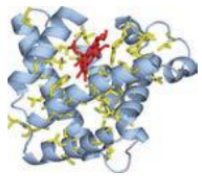
\includegraphics[width=3.5cm]{prot}}
	\subfigure{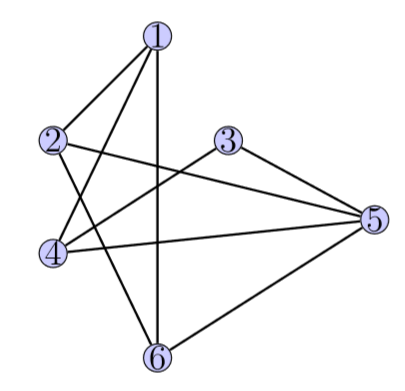
\includegraphics[width=3.5cm]{grafos}}
	\\
	\vspace{-0.2cm}
	\subfigure{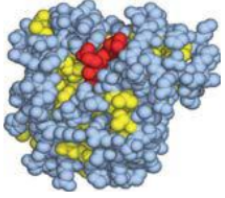
\includegraphics[width=3.7cm]{prot2}}
\end{figure}
\end{frame}


\section{Complexidade Computacional}
%SLIDE 2
\begin{frame}
\frametitle{\normalsize Preliminares}
	\large \textbf{Teoria de Complexidade Computacional}
	\\
	\normalsize \vspace{0.2cm} Trata-se da \textit{contagem de operações} necessárias para solucionar um problema, que podem variar abruptamente de caso a caso.
	\\ \vspace{0.3cm}Nos preocupamos em estudar os seguintes:
\begin{itemize}
	\item Melhor Caso
	\item Pior Caso
	\item Caso Médio
\end{itemize}

\vspace{0.2cm}\large Notação \textbf{Big O}
\\\vspace{0.2cm}\normalsize $T(n) = n^3 + 7n^2+ 40\ln{(n)}^3 \Rightarrow T(n) = O(n^3)$


\vspace{-2cm}
\begin{figure}
	\begin{flushright}
	\subfigure{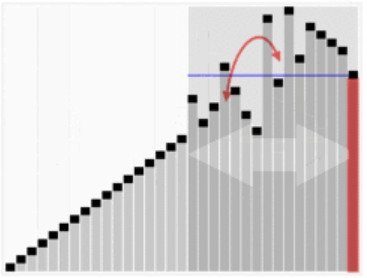
\includegraphics[width=4.0cm]{quicksort}}
	\end{flushright}
\end{figure}
\end{frame}

%SLIDE 3
\section{Modelando o Problema}
\begin{frame}
\frametitle{\normalsize Modelando o Problema}
\begin{multicols}{2}
	\textbf{Quais são as Entradas?}
	\begin{itemize}
    	\item Quantidade $n$ de átomos;
	   	\item Sequência teórica de átomos;
   		\item Distância teórica entre átomos;
   		\item Distância real entre átomos;
	\end{itemize}
 	\columnbreak
 	\textbf{Quais são as Saídas?}
 	\begin{itemize}
 		\item Posições $x_1, ..., x_n \in \mathbb{R}^3$ dos $n$ átomos da molécula.
 	\end{itemize}		    
\end{multicols}
Perceba, as distâncias reais contém incertezas associadas, logo, a RMN trás \textit{distâncias intervalares} da forma: $[\underline{d_{i,j}}, \overline{d_{i,j}}]$, ou seja
$$0\leq\underline{d_{i,j}}\leq d_{i,j} \leq \overline{d_{i,j}}$$
\end{frame}

%Slide 4
\section{Analise de um Caso Particular}
\begin{frame}
\frametitle{\normalsize Analisando um Caso Particular}
\vspace{-1.5cm}
Considere um \textbf{PGDM} \textbf{plano}, onde temos um grafo $V(G)=\{u, v, r, s\}$ e $E(G)=\{\{u,v\}, \{u, r\}, \{v, r\}, \{v, s\}, \{r, s\}, \{u, s\}\}$. \textbf{Fixando} \textit{u, v, r}, ou seja, \textbf{determinando} $ x_{u}, x_{v},x_{r} \in\mathbb{R}^2$ de tal modo que $\|x_{u} - x_{v}\|= d_{uv}$,  $\|x_{u} - x_{r}\|= d_{ur}$ e $\|x_{v} - x_{r}\|= d_{vr}$, podemos montar o  seguinte sistema quadrático:\vspace{0.50cm}
$$ \|x_{s} - x_{u}\|= d_{us} $$$$ \|x_{s} - x_{v}\|= d_{vs} $$$$ \|x_{s} - x_{r}\|= d_{rs} $$
\end{frame}

%Slide 5
\begin{frame}
\frametitle{\normalsize Analisando um Caso Particular}
Elevando os termos ao quadrado,
\vspace{-0.2cm}
$$\|x_{s}\|^{2} - 2(x_{s}.x_{u}) + \|x_{u}\|^{2} = d_{us}^{2}$$
\vspace{-0.7cm}$$\|x_{s}\|^{2} - 2(x_{s}.x_{v}) + \|x_{v}\|^{2} = d_{vs}^{2}$$
\vspace{-0.6cm}$$\|x_{s}\|^{2} - 2(x_{s}.x_{r}) + \|x_{r}\|^{2} = d_{rs}^{2}$$
subtraindo a primeira equação das outras duas, temos:
$$2(x_{s}.x_{v}) - 2(x_{s}.x_{u}) = \|x_{v}\|^{2} - \|x_{u}\|^{2} + d_{us}^{2} - d_{vs}^{2}$$
$$2(x_{s}.x_{r}) - 2(x_{s}.x_{u}) = \|x_{r}\|^{2} - \|x_{u}\|^{2} + d_{us}^{2} - d_{rs}^{2}$$
Colocando $x_{s}$ em evidência para ficar claro as incógnitas
$$2(x_{v} - x_{u})x_{s} = \|x_{v}\|^{2} - \|x_{u}\|^{2} + d_{us}^{2} - d_{vs}^{2}$$
$$2(x_{r} - x_{u})x_{s} = \|x_{r}\|^{2} - \|x_{u}\|^{2} + d_{us}^{2} - d_{rs}^{2}$$

Por tanto, temos um sistema linear $Ax = b$
\end{frame}

%Slide 5
\begin{frame}
\frametitle{\normalsize Analisando um Caso Particular}
$$
A = 2\begin{bmatrix}
x_{v1} - x_{u1} & x_{v2} - x_{u2}\\
x_{r1} - x_{u1} & x_{r2} - x_{u2}
\end{bmatrix}
$$
$$
b = \begin{bmatrix}
\|x_{v}\|^{2} - \|x_{u}\|^{2} + d_{us}^{2} - d_{vs}^{2}\\
\|x_{r}\|^{2} - \|x_{u}\|^{2} + d_{us}^{2} - d_{rs}^{2}
\end{bmatrix}
$$
$$
x = \begin{bmatrix}
x_{s1}\\
x_{s2}
\end{bmatrix}
$$

Perceba que se A for inversível, temos uma única solução $x^{*} = A^{-1}b$
\end{frame}

%Slide 6
\begin{frame}
\frametitle{\normalsize Analisando um Caso Particular}
\begin{center}
\textbf{Conclusão:} Se o grafo G de um \textbf{PGDM for completo}, então podemos resolver o problema através da resolução de\textbf{ N sistemas lineares}, sendo N proporcional ao numero de vértices.
\end{center}
\end{frame}

%Slide 6
\begin{frame}
\frametitle{\normalsize Analisando um Caso Particular}
\begin{center}
	\textbf{Conclusão:} Se o grafo G de um \textbf{PGDM for completo}, então podemos resolver o problema através da resolução de\textbf{ N sistemas lineares}, sendo N proporcional ao numero de vértices.
\end{center}

\large Dizemos então que o problema \textit{pode} ser resolvido em \textbf{tempo linear} \vspace{-0.2cm}\center \color{red}O(n)
\end{frame}

%Slide 6
\begin{frame}
\frametitle{\normalsize Analisando um Caso Particular}
\begin{center}
\textbf{Conclusão:} Se o grafo G de um \textbf{PGDM for completo}, então podemos resolver o problema através da resolução de\textbf{ N sistemas lineares}, sendo N proporcional ao numero de vértices.
\end{center}

\large Dizemos então que o problema \textit{pode} ser resolvido em \textbf{tempo linear} \vspace{-0.2cm}\center \color{red}O(n)
\color{black}
\\\vspace{1cm}
Infelizmente isso não acontece. O grafo molecular não é completo.
\end{frame}

%Slide 7
\section{Complexidade do PGDM}
\begin{frame}
\frametitle{\normalsize Analisando o caso Geral}
Para verificar a complexidade do PGDM nos resta olhar para a \textbf{otimização global} de
$$ f(x_1, ...,x_n) = \sum_{(i,j) \in E} (\|x_i - x_j\| - d_{ij})^2$$
por tanto:
$$ \min_{x_t \in\mathbb{R}^n} f(x_1, ...,x_n)$$
\end{frame}

%Slide 7
\begin{frame}
\frametitle{\normalsize Analisando o caso Geral}
Para verificar a complexidade do PGDM nos resta olhar para a \textbf{otimização global} de
$$ f(x_1, ...,x_n) = \sum_{(i,j) \in E} (\|x_i - x_j\| - d_{ij})^2$$
por tanto:
$$ \min_{x_t \in\mathbb{R}^n} f(x_1, ...,x_n)$$
\\\vspace{0.2cm}Infelizmente \textbf{tal minimização é inviável}, a quantidade de mínimos locais cresce \textbf{exponencialmente} com $n$.
\end{frame}

%Slide 8
\begin{frame}
\frametitle{\normalsize Analisando o caso Geral}
\center\large\textbf{Conclusão:} O custo computacional para resolver um PGDM que, suponha, todas as distâncias da RMN são precisas e que de fato representam as distâncias entre os átomos pode ser proporcional a $2^{\|v\|}$.
\end{frame}

%Slide 8
\begin{frame}
\frametitle{\normalsize Analisando o caso Geral}
\center\large\textbf{Conclusão:} O custo computacional para resolver um PGDM que, suponha, todas as distâncias da RMN são precisas e que de fato representam as distâncias entre os átomos pode ser proporcional a $2^{\|v\|}$.
\\\flushleft Logo,
\begin{teo}
O PGDM é um problema \textit{NP-Difícil}.
\end{teo}
\end{frame}

%Slide End
\begin{frame}
\centering
\begin{minipage}{0.3\linewidth}
	\begin{flushleft}
		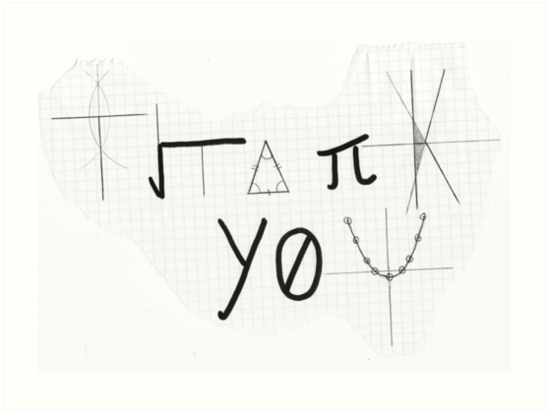
\includegraphics[scale=0.35]{thank}
	\end{flushleft}
\end{minipage}
\hspace{2.5cm}
\begin{minipage}{0.4\linewidth} \centering 
	{\color{blue} \underline{guilherme.philippi@hotmail.com}} \vspace{0.2cm}  \\ UFSC - Blumenau
\end{minipage}
\end{frame}

\end{document}